The representation of proteins shown in the structure diagram of
Figure \ref{fig:amino_connect} is suitable for determining the
chemical properties of the molecules, getting an overview of how atoms
are arranged and how the atoms are connected. However, to get an exact
model of the protein structure we need a lot more precision in our
characterization. That is, we need to include the concepts of bond
lengths, bond angles and torsional angles into the model. 

% Refer to
% Figure \ref{fig:protein-torsion-angles} while reading the following
% explanation of these concepts.

\section{Backbone geometry}
\textit{Bond lengths} are the distances between the individual atoms
in a molecule (usually measured in Ångstrøm). We will name the
individual bond lengths by the name of the two atoms which the bond
connects, e.g. the bond between a \Ca\ and N atom in an amino acid of
the protein backbone is called \Ca -N. We have computed bond lengths
for all bonds in the backbone, the results are shown in Table
\ref{tab:average_bond_lengths}. As can be seen from the last column in
the table, the variation is very constrained and we therefore havenøt
found it necessary to consider making any variations from the mean
lengths. 
%% Actually, these variations are so small that they can very possibly
%% be attributed to uncertainty in the measuring equipment.

\begin{table}
  \centering
  \begin{tabular}{lrr}
    \toprule
    \multicolumn{1}{c}{Bond} & \multicolumn{1}{c}{Avg. length} & \multicolumn{1}{c}{Std.dev.} \\ \midrule 
    C-O   & 1.2260 Å & 0.0188 Å\\
    CA-C  & 1.5272 Å & 0.0191 Å\\
    N-CA  & 1.4680 Å & 0.0237 Å\\
    C-N   & 1.3234 Å & 0.0215 Å\\
    N-H   & 0.9793 Å & 0.0342 Å\\
    CA-CB & 1.5327 Å & 0.0228 Å\\
    CA-HA & 1.0747 Å & 0.0307 Å\\ \bottomrule
  \end{tabular}
  \vspace{1mm}
  \caption{Average bond lengths (in ångstrøm)}
  \label{tab:average_bond_lengths}
\end{table}

A \textit{bond angle} is an angle between two outgoing bonds from a
single atom. As an example, the angle between the bonds N-\Ca\ and \Ca
-C' is called N-\Ca -C'. Table \ref{tab:average_bond_angles} shows
average values for the backbone bond angles in degrees. Again can we
see that the variation is very limited, but as a small angular
displacement can have a rather large influence on the remaining part
of the protein, they could still introduce variability into the model
of much larger order. In this project we have however selected to
focus solely on the variability in the torsional angles, thus locking
the bond angles to their mean values.

\begin{table}
  \centering
  \begin{tabular}{l>{$}r<{^\circ$}>{$}r<{^\circ$}}
    \toprule
    \multicolumn{1}{c}{Bond} & \multicolumn{1}{c}{Avg. angle} & \multicolumn{1}{c}{Std.dev.} \\ \midrule 
    H-N-CA & 118.9553 & 1.9979\\
    N-CA-C & 110.6099 & 2.4668\\
    CA-C-O & 120.7088 & 1.3064\\
    CA-C-N & 116.7804 & 1.7682\\
    C-N-CA & 121.4547 & 1.9946\\
    C-N-H  & 119.5112 & 2.1599\\ \bottomrule
  \end{tabular}
  \vspace{1mm}
  \caption{Average bond angles (in degrees)}
  \label{tab:average_bond_angles}
\end{table}


\begin{figure*}
  \centering
  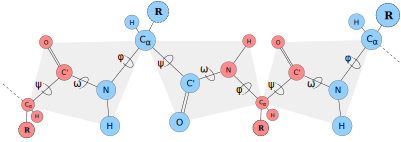
\includegraphics[width=0.75\textwidth]{figures/protein-torsion-angles}
  \caption{Illustration of the protein torsion angles in a protein sequence extract.}
  \label{fig:protein-torsion-angles}
\end{figure*}

A \textit{torsional angle} is rotational angle around a bond. In the
backbone, there are three of such torsional angles (see Figure
\ref{fig:protein-torsion-angles}). The $\phi$ and $\psi$ angles were
mentioned earlier and we will return to them after this paragraph. The
last one, the $\omega$-angle, is almost always $180^{\circ}$
\cite{probik}, but at a few occurrences it deviates from this
value. We will assume that the $\omega$ angle is \textit{always}
$180^{\circ}$. This makes the grey rectangular areas of Figure
\ref{fig:protein-torsion-angles} completely rigid.  Each of the
torsional angles can be defined as dihedral angles between two
planes. For example, the $\phi$ angle can be described by the angle
between the two planes defined by the atoms C'$_{n-1}$, N$_n$ and \Ca
$_n$ as well as N$_n$, \Ca $_n$ and C'$_n$.

Getting back to the $\phi$ and $\psi$, we can now see that these are
the main variability of the protein backbone, as all bond lengths and
bond angles are nearly rigid and the $\omega$-angle has rarely
deviates from the $180^\circ$ value. 

Because of collisions between side-chains and the backbone, only
certain combinations of $\phi$ and $\psi$ angles are legal. The legal
angles can be illustrated graphically in what is known as a
\textit{Ramachandran plot} (Figure \ref{fig:ramachandran}). In the
plot on the left (Figure \ref{fig:ramachandran}) legal values for all
amino acids except Glycine has been shown. And in the right plot legal
values for Glycine has been shown. Glycine is special because of its
simplicity. It consists of a single H atom connected to the $C_\alpha$
of the amino acid and thus collisions with the backbone is hardly a
problem.

\begin{figure*}
	\centering
	\subbottom[]{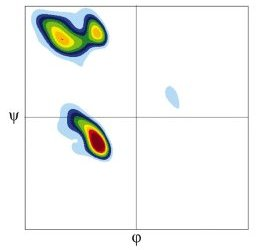
\includegraphics[width=0.3\textwidth]{figures/ramachandran_except_gly} \label{fig:ramachandran}}
    \subbottom[]{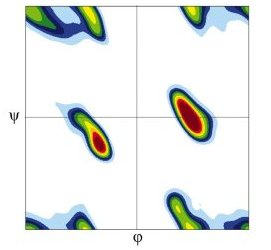
\includegraphics[width=0.3\textwidth]{figures/ramachandran_only_gly} \label{fig:ramachandran_gly}}
    \caption{\textbf{(a)} A ramachandran plot for all amino
      acids except Glycine. \textbf{(b)}  Ramachandran plot
      for Glycine. The figure is from Wikipedia, licensed under Creative Commons.}
\end{figure*}

\section{Side-chain geometry}
Rotamers (evt. calculating bond angles and bond lengths)
